\chapter{What Changes in the Real World}

\begin{tldr}
\begin{itemize}
  \item \textbf{Last chapter:} parasitic files (ITF, mapping, SPEF) told the tool what each routed wire actually does electrically. \textbf{This chapter:} we zoom out and see how every input covered so far explodes in production: MMMC view counts, pin access, derate models, and DEF size growth through the flow.
  \item \textbf{MMMC is multiplication, not addition.} Five cell families times three voltages times three temperatures times six process corners times four modes is not a clever rhetorical flourish; it is a literal \texttt{.lib} count north of one thousand.
  \item \textbf{Pin access is the new floorplan.} At 7\,nm, an instance can be DRC-clean in placement and still strand the router because the M1 pin geometry offers too few via-cut candidates.
  \item \textbf{OCV, AOCV, POCV change the answer on the same SDC.} A path that meets timing at 1.05\,ns with AOCV can fail at 1.10\,ns with flat OCV without a single edit to the constraint file.
\end{itemize}
\end{tldr}

\begin{hook}
A junior engineer hands you a netlist, a tech file, an SDC, a LEF, a Liberty, and a DEF. You set up the run. The tool refuses to launch. The error is one line: \texttt{ERROR: analysis\_view 'func\_ss\_0p72\_125c\_setup' references missing delay\_corner}. You did not forget a file. You forgot that the toy version of every input you just read about explodes into a matrix of views the moment the block is real. So what does the matrix actually look like, and where does the explosion bite first?
\end{hook}

% =====================================================================
\section{MMMC: the Liberty view explosion}
% =====================================================================

The toy mental model says ``load a \texttt{.lib}, load an SDC, run STA.'' The production model says ``enumerate every physically possible combination of process, voltage, temperature, cell flavor, and operating mode, then promise the foundry your design works at every cross product.'' That promise is what \textbf{MMMC} (Multi-Mode Multi-Corner) signoff actually encodes.

\subsection{Counting the Liberty views directly}

Walk through it with the numbers in front of you. The arithmetic is boring; the size of the answer is not.

\move{1} \textbf{Cell families.} A modern 7\,nm-class standard cell library ships in five threshold flavors: \textbf{RVT, LVT, HVT, ULVT, ELVT}. That is \textbf{5}.

\move{2} \textbf{Voltages.} Each flavor is characterized at \textbf{nominal, low, and overdrive}. That is \textbf{3}.

\move{3} \textbf{Temperatures.} Automotive-aware blocks characterize at \textbf{$-40^\circ$C, $25^\circ$C, $125^\circ$C}. That is \textbf{3}.

\move{4} \textbf{Process corners.} Setup signoff uses \textbf{SS, FF, TT, SF, FS}, and hold typically demands a second \textbf{FS variant} with a separate skew assumption. That is \textbf{6}.

\move{5} \textbf{Operating modes.} The block runs in \textbf{functional, scan-shift, scan-capture, and retention} modes. That is \textbf{4}.

\move{6} \textbf{Multiply.} $5 \times 3 \times 3 \times 6 \times 4 = \mathbf{1080}$ Liberty views. The chapter's old ``easily exceeds 200'' was a comforting understatement.

\move{7} \textbf{Wall-clock cost.} Liberty parsing scales roughly linearly. At \textbf{30 seconds per view}, parsing alone is $1080 \times 30 = 32{,}400$ seconds, or \textbf{nine hours} if you do it serially. In practice tools cache and parallelize, but the order of magnitude is real, and every parse hits disk.

\begin{keyidea}
The MMMC view count is the \textbf{product} of every characterization axis, not the sum. Adding a single new voltage point does not add one view; it multiplies the entire existing matrix by a new factor.
\end{keyidea}

\subsection{How Innovus actually structures it}

Innovus does not consume 1080 raw Liberty files as 1080 independent things. It organizes them into three objects that compose:

\begin{itemize}
  \item \textbf{library\_set}: a bundle of \texttt{.lib} files that belong together (one PVT corner across all cell families).
  \item \textbf{delay\_corner}: a library\_set plus an RC corner (the QRC tech file) plus an OCV derate spec.
  \item \textbf{constraint\_mode}: an SDC file plus the mode it represents (functional, scan, retention).
  \item \textbf{analysis\_view}: the actual scenario you sign off, formed by pairing one \texttt{constraint\_mode} with one \texttt{delay\_corner}.
\end{itemize}

The number that matters at runtime is not the 1080 Liberty views; it is the \textbf{number of analysis\_views you activate}. A typical 7\,nm block runs signoff on roughly \textbf{20 to 40 active views} simultaneously, picked from the full matrix to cover worst setup, worst hold, worst leakage, and the mode-specific corners. The full 1080 is the universe; the active set is the working slice.

\begin{hook}
\textbf{The Liberty matrix is a warehouse, the analysis\_view list is the loading dock.} If you forget which crates you actually shipped today, signoff signs off on the wrong block and the tapeout slips a month.
\end{hook}

\begin{gut}
A block uses 4 cell families, 2 voltages, 2 temperatures, 5 process corners, and 3 modes. How many Liberty views, and how is the \emph{analysis\_view} number different from that?
\gutans{$4 \times 2 \times 2 \times 5 \times 3 = 240$ Liberty views. The analysis\_view count is whatever subset of (constraint\_mode $\times$ delay\_corner) you actually activate for signoff, typically 15 to 30 in production. The matrix sizes the disk; the active list sizes the runtime.}
\end{gut}

% =====================================================================
\section{Pin access: when LEF stops being enough}
% =====================================================================

At 28\,nm, a standard cell's LEF \texttt{PIN} section drew an M1 rectangle spanning the cell width. The router saw a long target, dropped a via almost anywhere along it, and moved on. At 7\,nm that same geometry strands the router, and placement legality stops implying routability.

\subsection{Why the 28\,nm pin shape fails at 7\,nm}

\move{1} \textbf{Track pitch.} A 7\,nm M1 routing pitch is roughly \textbf{36\,nm}. The router can only place a wire on one of those tracks; nothing in between is legal.

\move{2} \textbf{Pin geometry must land on a track.} A pin rectangle whose center sits between two tracks is invisible to the router. The cell can be placed, but no legal wire can touch it.

\move{3} \textbf{Via cuts are quantized.} A 7\,nm V1 cut is roughly $32 \times 32$\,nm and must obey same-cut spacing. A pin shape that is only \textbf{one track wide} offers \textbf{one via candidate}. If that candidate clashes with a neighbor cell's via, the router has zero alternatives.

\move{4} \textbf{Multi-access pins.} Modern foundry cell libraries require each input pin to offer at least \textbf{two non-conflicting via candidates}, sometimes three. This is enforced by a separate deliverable.

\move{5} \textbf{Pin access models.} The foundry ships a \textbf{pin access model} (often a CSV or proprietary table per cell) listing which access points are usable under which neighbor contexts. It augments the LEF; it does not replace it.

\begin{figure}[h]
\centering
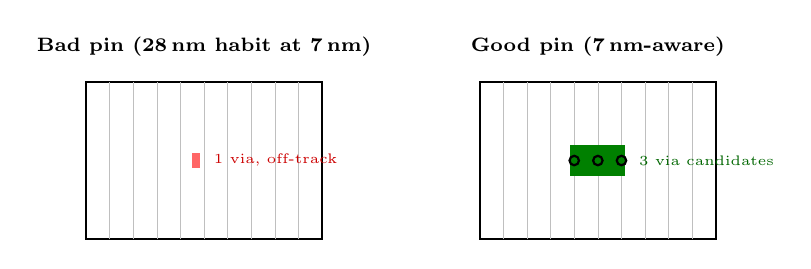
\begin{tikzpicture}[font=\scriptsize]
  % BAD pin
  \begin{scope}
    \node[anchor=south, font=\scriptsize\bfseries] at (1.5,2.2) {Bad pin (28\,nm habit at 7\,nm)};
    % cell outline
    \draw[thick] (0,0) rectangle (3,2);
    % tracks
    \foreach \x in {0.3,0.6,0.9,1.2,1.5,1.8,2.1,2.4,2.7} {
      \draw[gray!50, very thin] (\x,0) -- (\x,2);
    }
    % pin shape (between tracks, narrow)
    \fill[red!60] (1.35,0.9) rectangle (1.45,1.1);
    \node[red!80!black, anchor=west, font=\tiny] at (1.5,1.0) {1 via, off-track};
  \end{scope}

  % GOOD pin
  \begin{scope}[xshift=5cm]
    \node[anchor=south, font=\scriptsize\bfseries] at (1.5,2.2) {Good pin (7\,nm-aware)};
    \draw[thick] (0,0) rectangle (3,2);
    \foreach \x in {0.3,0.6,0.9,1.2,1.5,1.8,2.1,2.4,2.7} {
      \draw[gray!50, very thin] (\x,0) -- (\x,2);
    }
    % pin spans three tracks, on-grid
    \fill[green!50!black] (1.15,0.8) rectangle (1.85,1.2);
    \foreach \x in {1.2,1.5,1.8} {
      \draw[black, thick] (\x,1.0) circle (0.06);
    }
    \node[green!40!black, anchor=west, font=\tiny] at (1.9,1.0) {3 via candidates};
  \end{scope}
\end{tikzpicture}
\caption{Pin access geometry at 7\,nm. The left pin is on-grid for placement but off-grid for routing tracks and offers a single via candidate; the router has no fallback when the neighbor cell wants the same cut. The right pin spans three tracks and offers three independent via candidates.}
\end{figure}

\begin{pitfall}
``Placement DRC clean'' at 7\,nm does \textbf{not} mean ``routable.'' A block can finish placement with zero violations and then accumulate thousands of \textbf{unconnected nets} in detail route because of pin-access conflicts the placer never modeled. Always check the pin-access report before signing off on a placement milestone.
\end{pitfall}

% =====================================================================
\section{AOCV and POCV: same SDC, different answer}
% =====================================================================

The SDC defines the constraints. The derate model defines how pessimistic the tool is when it applies those constraints. Three derate models dominate production today: \textbf{flat OCV}, \textbf{AOCV} (Advanced OCV, depth-aware), and \textbf{POCV} (Parametric OCV, statistical).

\subsection{Worked example: a 12-level path at 1.0\,ns nominal}

The path has \textbf{12 logic levels} (12 cells on the data path between launch and capture flops). Nominal cell-plus-net delay sums to \textbf{1.0\,ns}. The clock period is 1.05\,ns.

\move{1} \textbf{Flat OCV.} The launch path is derated up by 1.10, the capture path down by 0.90. Launch delay becomes $1.0 \times 1.10 = \mathbf{1.10\,\text{ns}}$. With a 1.05\,ns period the path \textbf{misses by 50\,ps}.

\move{2} \textbf{AOCV table lookup.} The AOCV table is depth-dependent: \textbf{1.15} at depth 1, \textbf{1.05} at depth 12, with linear interpolation between. The longer the path, the less pessimism, because statistical variation of independent stages partially cancels.

\move{3} \textbf{AOCV applied.} At depth 12 the multiplier is \textbf{1.05}. Launch delay is $1.0 \times 1.05 = \mathbf{1.05\,\text{ns}}$. The path \textbf{just meets} the 1.05\,ns period.

\move{4} \textbf{POCV per-cell sigma.} Each cell publishes a $\sigma/\mu$ ratio in a \texttt{.lib} extension. Assume the 12 cells contribute equal mean delay (83.3\,ps each) and each has $\sigma/\mu = 0.05$. Per-cell $\sigma = 0.05 \times 83.3 = 4.17$\,ps.

\move{5} \textbf{POCV sqrt-sum-of-squares.} Path $\sigma = \sqrt{12 \times 4.17^2} = \sqrt{208.7} = \mathbf{14.4\,\text{ps}}$. The path mean is 1.000\,ns.

\move{6} \textbf{POCV signoff (mean + $3\sigma$).} Launch delay is $1.000 + 3 \times 0.0144 = 1.000 + 0.043 = \mathbf{1.043\,\text{ns}}$. The path meets with \textbf{7\,ps of margin}, more than AOCV gave you.

\move{7} \textbf{Tally.}
\begin{itemize}
  \item Flat OCV: 1.10\,ns, \textbf{fails by 50\,ps}.
  \item AOCV: 1.05\,ns, \textbf{meets by 0\,ps}.
  \item POCV: 1.043\,ns, \textbf{meets by 7\,ps}.
\end{itemize}

Same SDC. Same netlist. Same instance placement. Three different signoff verdicts because the derate engine changed.

\begin{pausebox}
Halfway recap. MMMC says ``how many corners.'' Pin access says ``can the router even reach.'' OCV/AOCV/POCV says ``how mean is the signoff math.'' All three modify outputs the SDC and Liberty already promised, so the toy mental model of ``one .lib, one SDC, one answer'' is a story the production flow does not tell.
\end{pausebox}

\begin{gut}
The same 12-level path under flat OCV fails by 50\,ps; under POCV it passes with 7\,ps margin. Did the silicon get faster?
\gutans{No. The silicon did not change. The \textbf{statistical model of how variation accumulates} changed. Flat OCV assumes every stage hits its worst case simultaneously, which becomes wildly pessimistic as path depth grows; POCV models that independent stages partially cancel and reports a tighter, more physically realistic margin.}
\end{gut}

% =====================================================================
\section{DEF growth through the flow, with post-CTS as the surprise}
% =====================================================================

DEF is the same file format at every PD checkpoint, but the byte count tells a story about what each stage added. The post-CTS jump is the one new engineers miss, because the netlist itself changed underneath them.

\subsection{Worked example: a 1M-instance block}

Take a 1\,million-instance block and follow the DEF through the flow.

\move{1} \textbf{Post-floorplan.} DEF holds \texttt{DIEAREA}, \texttt{ROWS}, IO pin placement, and macro placement. Standard cells are not placed; \texttt{COMPONENTS} lists them with placeholder status. Size: \textbf{$\sim$30\,MB}.

\move{2} \textbf{Post-place.} Every one of the 1\,M instances now has an \texttt{(x, y)} coordinate and an orientation. Each \texttt{COMPONENT} line grows by roughly 40\,bytes. Net topology has not been written yet. Size: \textbf{$\sim$80\,MB}.

\move{3} \textbf{Post-CTS.} The CTS engine \textbf{inserted new instances}, roughly \textbf{5\% of the original count}, as clock buffers, inverters, and ICGs. That is \textbf{50\,000 new components}. It also \textbf{rewrote every clock \texttt{NET}} to reflect the new tree topology. Size: \textbf{$\sim$120\,MB}.

\move{4} \textbf{Post-route.} Every \texttt{NET} now carries full routing geometry: \texttt{ROUTED} segments with layer, coordinates, and via instances. Average net contributes 200 to 400 bytes of geometry. Size: \textbf{$\sim$350\,MB}.

\move{5} \textbf{The post-CTS diff is the most informative diff in the flow.} Run \texttt{diff post\_place.def post\_cts.def}. The only changes you should see are (a) new clock-buffer \texttt{COMPONENT} entries and (b) rewritten clock \texttt{NET} entries. If you see signal nets change, CTS touched something it should not have.

\begin{figure}[h]
\centering
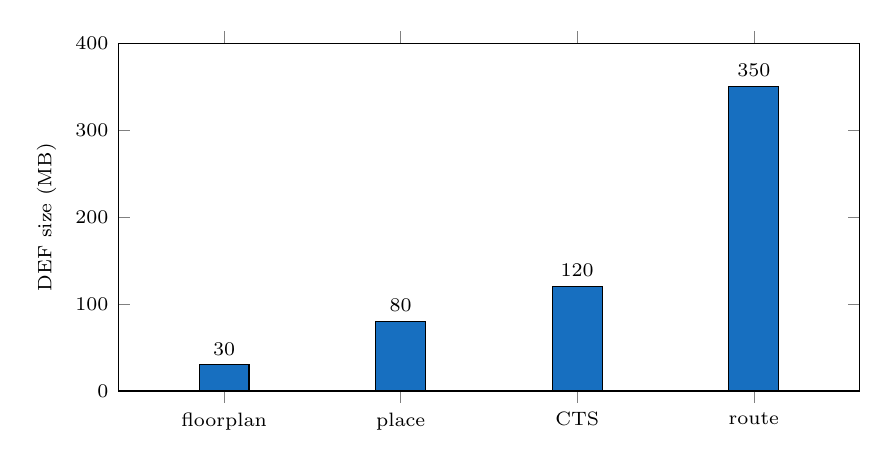
\begin{tikzpicture}
\begin{axis}[
  width=11cm, height=6cm,
  ybar,
  bar width=18pt,
  ylabel={DEF size (MB)},
  symbolic x coords={floorplan, place, CTS, route},
  xtick=data,
  nodes near coords,
  nodes near coords style={font=\scriptsize},
  ymin=0, ymax=400,
  enlarge x limits=0.2,
  tick label style={font=\scriptsize},
  label style={font=\scriptsize},
]
\addplot[fill=cyan!50!blue, draw=black] coordinates {(floorplan,30) (place,80) (CTS,120) (route,350)};
\end{axis}
\end{tikzpicture}
\caption{DEF size growth across PD stages for a 1\,M-instance 7\,nm block. The post-place to post-CTS jump (+40\,MB) reflects 50\,000 inserted clock instances and rewritten clock NETs. The post-route jump (+230\,MB) is dominated by per-net routing geometry.}
\end{figure}

\begin{hook}
\textbf{The post-CTS DEF gains 40\,MB and 50\,000 instances overnight; if you do not diff it against post-place, you will not notice when CTS quietly buffered a signal net and your scan chain breaks at silicon.}
\end{hook}

\begin{sidebar}
Why does the post-route jump dwarf everything else? Because routing geometry is the only DEF content that scales with \textbf{net length in microns}, not with \textbf{instance count}. A single long bus net on M5 can contribute as much DEF text as a hundred short local nets. This is also why \texttt{def2stream} for GDS conversion is the slowest step in the back-end: it is parsing geometry, not instances.
\end{sidebar}

% =====================================================================
\section{Why PD Cares}
% =====================================================================

\begin{pdnote}[Why PD Cares]
\textbf{Arm PD intern lens (you, this summer on Duc):} you will load MMMC views in your first week, and the first error will be a missing \texttt{analysis\_view} reference in the Innovus setup script. Knowing that \texttt{analysis\_view = constraint\_mode $\times$ delay\_corner} is what unblocks you in fifteen minutes instead of two days. You will also spend serious time staring at post-CTS DEF diffs because Duc is CTS-heavy.\\
\textbf{Generic PD engineer lens:} when a tool ``runs out of memory'' or ``hangs on STA setup,'' the answer is almost always MMMC scenario explosion or a derate file mismatch, not an algorithmic regression. Check the view count first.\\
\textbf{VLSI interview lens:} expect ``what is the difference between OCV, AOCV, and POCV, and when would you use each?'' as a standard signoff-flow question. The right answer leads with the numbers (flat is most pessimistic, POCV is least pessimistic on long paths) and then names the formulas.
\end{pdnote}

% =====================================================================
\begin{checkpoint}
Production PD warps four inputs around the toy mental model: Liberty views \textbf{multiply}, pins must \textbf{align}, derate \textbf{rewrites the verdict}, and DEF \textbf{grows fastest at CTS and route}.
\mnemonic{Multiply, Align, Derate, Grow (MADG).}
\end{checkpoint}
